% \documentclass[aps,prl,preprint,groupedaddress]{revtex4-1}
%\documentclass[aps,prl,preprint,superscriptaddress]{revtex4-1}
\documentclass[aps,prl,reprint,superscriptaddress]{revtex4-1}
\newcommand{\SSC}{S/S_{c}}
\newcommand{\mnras}{Monthly Notices of the Royal Astronomical Society}
\newcommand{\apjs}{The Astrophysical Journal Supplement Series}
\usepackage{graphicx}
% You should use BibTeX and apsrev.bst for references
% Choosing a journal automatically selects the correct APS
% BibTeX style file (bst file), so only uncomment the line
% below if necessary.
%\bibliographystyle{apsrev4-1}

\begin{document}

% Use the \preprint command to place your local institutional report
% number in the upper righthand corner of the title page in preprint mode.
% Multiple \preprint commands are allowed.
% Use the 'preprintnumbers' class option to override journal defaults
% to display numbers if necessary
%\preprint{}

%Title of paper
\title{The Magnetorotational Instability Prefers Three Dimensions}

% repeat the \author .. \affiliation  etc. as needed
% \email, \thanks, \homepage, \altaffiliation all apply to the current
% author. Explanatory text should go in the []'s, actual e-mail
% address or url should go in the {}'s for \email and \homepage.
% Please use the appropriate macro foreach each type of information

% \affiliation command applies to all authors since the last
% \affiliation command. The \affiliation command should follow the
% other information
% \affiliation can be followed by \email, \homepage, \thanks as well.
\author{Jeffrey~S.~Oishi}
\email[]{joishi@bates.edu}
\affiliation{Bates College Department of Physics and Astronomy, Lewiston, ME 04240}

\author{Geoffrey~M.~Vasil}
\affiliation{University of Sydney School of Mathematics and Statistics, Sydney, NSW, Australia}
\author{Morgan Baxter}
\affiliation{Bates College Department of Physics and Astronomy, Lewiston, ME 04240}
\author{Andrew Swan}
\affiliation{Faculty of Mathematics, Cambridge University, Cambridge, United Kingdom}
\author{Keaton~J.~Burns}
\affiliation{Center for Computational Astrophysics, Flatiron Institute, New York, NY 10010}
\affiliation{Massachusetts Institute of Technology Department of Physics, Cambridge, MA 02139}
\author{Daniel~Lecoanet}
\affiliation{Princeton Center for Theoretical Science and Princeton University Department of Astrophysical Sciences, Princeton, NJ 08544}
\author{Benjamin~P.~Brown}
\affiliation{University of Colorado Laboratory for Atmospheric and Space Physics and Department of Astrophysical and Planetary Sciences, Boulder, CO 80309}

% 
%\homepage[]{Your web page}
%\thanks{}
%\altaffiliation{}


%Collaboration name if desired (requires use of superscriptaddress
%option in \documentclass). \noaffiliation is required (may also be
%used with the \author command).
%\collaboration can be followed by \email, \homepage, \thanks as well.
%\collaboration{}
%\noaffiliation

\date{\today}

\begin{abstract}
The magnetorotational instability (MRI) is a powerful instability in which conducting fluids with weak magnetic fields and decreasing angular velocity are linearly unstable.
The MRI is thought to be essential to the operation of astrophysical accretion disks, where the angular velocity graident is supplied by the gravitational field of the central object.
However, the MRI may also be important in the internal shear layers of stars, where the MRI may operate in a poorly studied regime where the shear is near critical but the dissipative forces are negligable.
Here, we consider the linear stability of three-dimensional perturbations to a nearly inviscid and ideal magnetofluid and show that the fastest growing modes are three dimensional when the instability is near onset.
These three dimensional modes are unstable at shear rates down to 0.10 $S_c$, the critical value in two dimensions, and they have growth rates exceeding the fastest two dimensional modes until the shear parameter is about $2.05 S_c$.
These modes are significant, as they suggest the possibility of direct dynamo action from the linear instability itself.
Furthermore, even when two dimensional modes have the fastest growth rates, significant numbers of three dimensional modes are unstable.
In such a system, the non-normal character of the MRI cannot be ignored anytime the shear is near critical.
Because evidence from weakly non-linear analysis suggests that the MRI saturates by pushing the shear rate to its critical value, non-normality is never unimportant for systems, like stars, that can rearrange their angular velocity profiles.
\end{abstract}

% insert suggested PACS numbers in braces on next line
\pacs{}
% insert suggested keywords - APS authors don't need to do this
%\keywords{}

%\maketitle must follow title, authors, abstract, \pacs, and \keywords
\maketitle

% body of paper here - Use proper section commands
% References should be done using the \cite, \ref, and \label commands

The magnetorotational instability (MRI) is an extremely important instability in astrophysical fluid dynamics.
By changing the stabiliity criterion for differentially rotating flows from a negative angular \emph{momentum} gradient to a negative angular \emph{velocity} gradient, a weak magnetic field allows the Keplerian velocity profile due to a central point mass to drive turbulence \citep[e.g.][]{1998RvMP...70....1B}.
This discovery provided a pathway to explain the ubiquitous accretion onto compact objects at rates compatible with observations and may play a significant role in the formation of planets \citep[e.g.][]{2007Natur.448.1022J}.
In these objects, the gravitational field dominates the local plasma dynamics, and thus the MRI cannot significantly affect the background shear.
It must saturate by other means in these situations \citep{2018MNRAS.474.3451X}.
However, stars and liquid metal Taylor-Couette expereiments have differential rotation profiles driven by much weaker stresses.
Where the MRI is active in these flows, it can sature by pushing the background shear close to critical \citep{2017ApJ...841....1C,2017ApJ...841....2C}, analogous to the saturation of convection by relaxing to a nearly constant entropy profile.
Stellar interiors are at extremely high fluid and magnetic Reynolds numbers, but may potentially operate at or near the critical shear rate for the MRI\@.
This critical shear is set by the background magnetic field strength for axisymmetric perturbations in a channel of a given size.
Despite the extensive literature on the accretion disk case of strong shear and high Reynolds numbers and the liquid metal literature on weak shear and lower Reynolds numbers, even the linear dynamics of the MRI are not well studied in the weak shear, high Reynolds number regime.

Here, we investigate the stability of three dimensional perturbations near the two dimensional critical shear rate $S_c$ for a nearly invisicd, ideal MHD flow.
We find that the first modes to become destabilized are three-dimensional and thus act as a dynamo even in the absence of secondary instability.
These results strongly suggest that the non-normality of the linear operator driving the MRI are always important, even when axisymmetric modes dominate.
% \begin{itemize}
% \item 3D $\to$ dynamo
% \item stars, NSSL
% \item experiments
% \item Squire's theorem violation? Check MHD Squire, check S instead of Re...
% \item Do eigenvalue solution for B growth? i.e.\ check if it is a dynamo?
% \end{itemize}

We solve the linearized magnetohydrodynamic equations in rotating plane Couette geometry.
This corresponds to a Cartesian frame rotating with angular frequency $\Omega$ and a linear background shear, $v_{y0} = Sx$. 
We cast the Navier-Stokes equation in a fairly standard form,
\begin{equation}
  \label{eq:ns}
  \frac{D \mathbf{v}}{Dt} - f \hat{z} \times \mathbf{v} + S v_x \hat{z} + \mathbf{\nabla}{p} + \nu \mathbf{\nabla} \times \mathbf{\omega} = 0,
\end{equation}
where $\omega = \mathbf{\nabla} \times \mathbf{v}$ is the vorticity, $f = 2 \Omega$ is the Coriolis parameter, and $S$ is the background shear rate.
It is common in the accretion disk literature to relate $S$ and $f$ via the $q = S/f$ parameter; for all runs here, $q = 0.75$.
$Df/Dt = \partial f/\partial t + S x \partial f/\partial y$ is the advective derivative including the background linear shear velocity.  We write the induction equation in terms of the $x$ component of the magnetic field,
\begin{equation}
  \label{eq:Bx}
  \frac{D B_x}{Dt} - B_0 \partial_z v_x + \eta (\partial_y J_z - \partial_z J_y) = 0
\end{equation}
and the $x$ component of the current density,
\begin{equation}
  \label{eq:Jx}
  \frac{D J_x}{Dt} - B_0 \partial_z \omega_x + S \partial_z B_x - \eta \nabla^2 J_x = 0
\end{equation}
We explicitly enforce the divergence constraint on the incompressible velocity field $v$ and the magnetic field,
\begin{equation}
  \label{eq:divu}
  \mathbf{\nabla} \cdot \mathbf{v} = \mathbf{\nabla} \cdot \mathbf{B} = 0.
\end{equation}
The magnetic field is expressed in Alfven units, $\mathbf{B} = \mathbf{B_*}/\sqrt{\mu_0 \rho}$.
We consider the behavior of the MRI in a vertically ($z$) and horizontally ($y$) periodic channel of width $d = \pi$. The walls at $x = \pm d/2$ are perfectly conducting and stress-free. The MRI is a weak-field instability; in the inviscid, ideal case the critical shear rate for instability in two dimensions is given by
\begin{equation}
  \label{eq:Sc}
  S_c = \frac{-\pi^2 B^2}{f d^2}.
\end{equation}
Here, we use $\SSC$ as our control parameter. 

We solve equations~(\ref{eq:ns})--~(\ref{eq:divu}) by assuming harmonic perturbations in $y$ and $z$, $f = \hat{f}(x) e^{i(k_y y + k_z z) + \sigma t}$, where $\sigma = \gamma + i\omega$ with $\gamma$ and $\omega$ real. This reduces to an eigenvalue problem in $x$, which we solve using the \emph{Dedalus} framework. The advantage of this particular form is that it can be expressed as a set of ten first-order equations with Dirichlet boundary conditions for the stress-free, perfect conductor boundary conditions we use. 
Our interest is in ideal ($\eta = 0$), inviscid ($\nu = 0$) conditions.
However, in order to avoid critical layers in the stable solutions, we set $\eta=\nu=10^{-5}$.
We have confirmed our main results are insensitive to this particular value. 
1For each $(k_y, k_z)$ pair, we solve an eigenvalue problem with $n_x = 128$ modes; our results are identical at double the resolution\footnote{All code used in this paper can be found at \protect\url{https://github.com/jsoishi/mri\_prefers\_3d}}.


Our main result is that at small values of supercriticality, the fastest growing mode is not axisymmetric. 
Figure~\ref{fig:growth_rate}a shows the growth rates for four values of $\SSC$. 
At $\SSC = 1.02$, the maximum growth rate is found at $(k_y, k_z) \simeq (0.263, 0.447)$.
In fact, the first panel of figure~\ref{fig:growth_rate}a shows $\SSC = 0.640$, where there are no unstable two-dimensional modes, but three-dimensional instability is present.
The critical shear for three dimensional perturbations is at $S_{c,3D} \simeq 0.
102 S_c$.

While surprising, that three-dimensional perturbations grow faster than two-dimensional ones can be predicted analytically.
By expanding equations~(\ref{eq:ns}-\ref{eq:divu}) in terms of $S = S_c + \epsilon R$, such that the shear is asymptotically close to the critical rate for two dimensional perturbations, we compute the leading order correction to the growth rate from three-dimensional effects as
\begin{widetext}
\begin{equation}
  \label{eq:asymp}
\sigma^{2} \ = -\frac{q\,B^{2}}{(q+1)} \left[ k_z^2 \left(\frac{d^2}{\pi^{2}} k_z^2-R\right) \ - \ \frac{\left(6+\pi ^2\right) q+\pi
   ^2-6}{12 } \, k_{y}^{2}  \right] \ + \ ...
\end{equation}
\end{widetext}
The first term in equation~(\ref{eq:asymp}) is the result from a two-dimensional calculation.
The second term is negative definite and proportional to $k_y^2$: for sufficiently large $k_y$, it leads to instability even when the two-dimensional modes are stable.

Figure~\ref{fig:growth_rate}b compares the numerically growth rates for $\SSC=1.002$ between $0 \le k_y \le 0.2$ to this asymptotic approximation, showing that the numerical calculations accurately reproduce the analytic ones in the region where the latter is valid.
We provide the full spectrum for the most unstable parameter values for $\SSC = 1.02$ in figure~\ref{fig:growth_rate}c.
The single unstable mode is purely growing (orange dot), and its complex conjugate is also present (blue dot at $\omega = 0$), consistent with equation~(\ref{eq:asymp}).
The other stable modes (blue dots) are rotationally modified Alfven waves found in left- and right- going pairs, consistent with the analytic predictions for two-dimensional stability calculations.
%
%\onecolumngrid

\begin{figure*}[h!]
  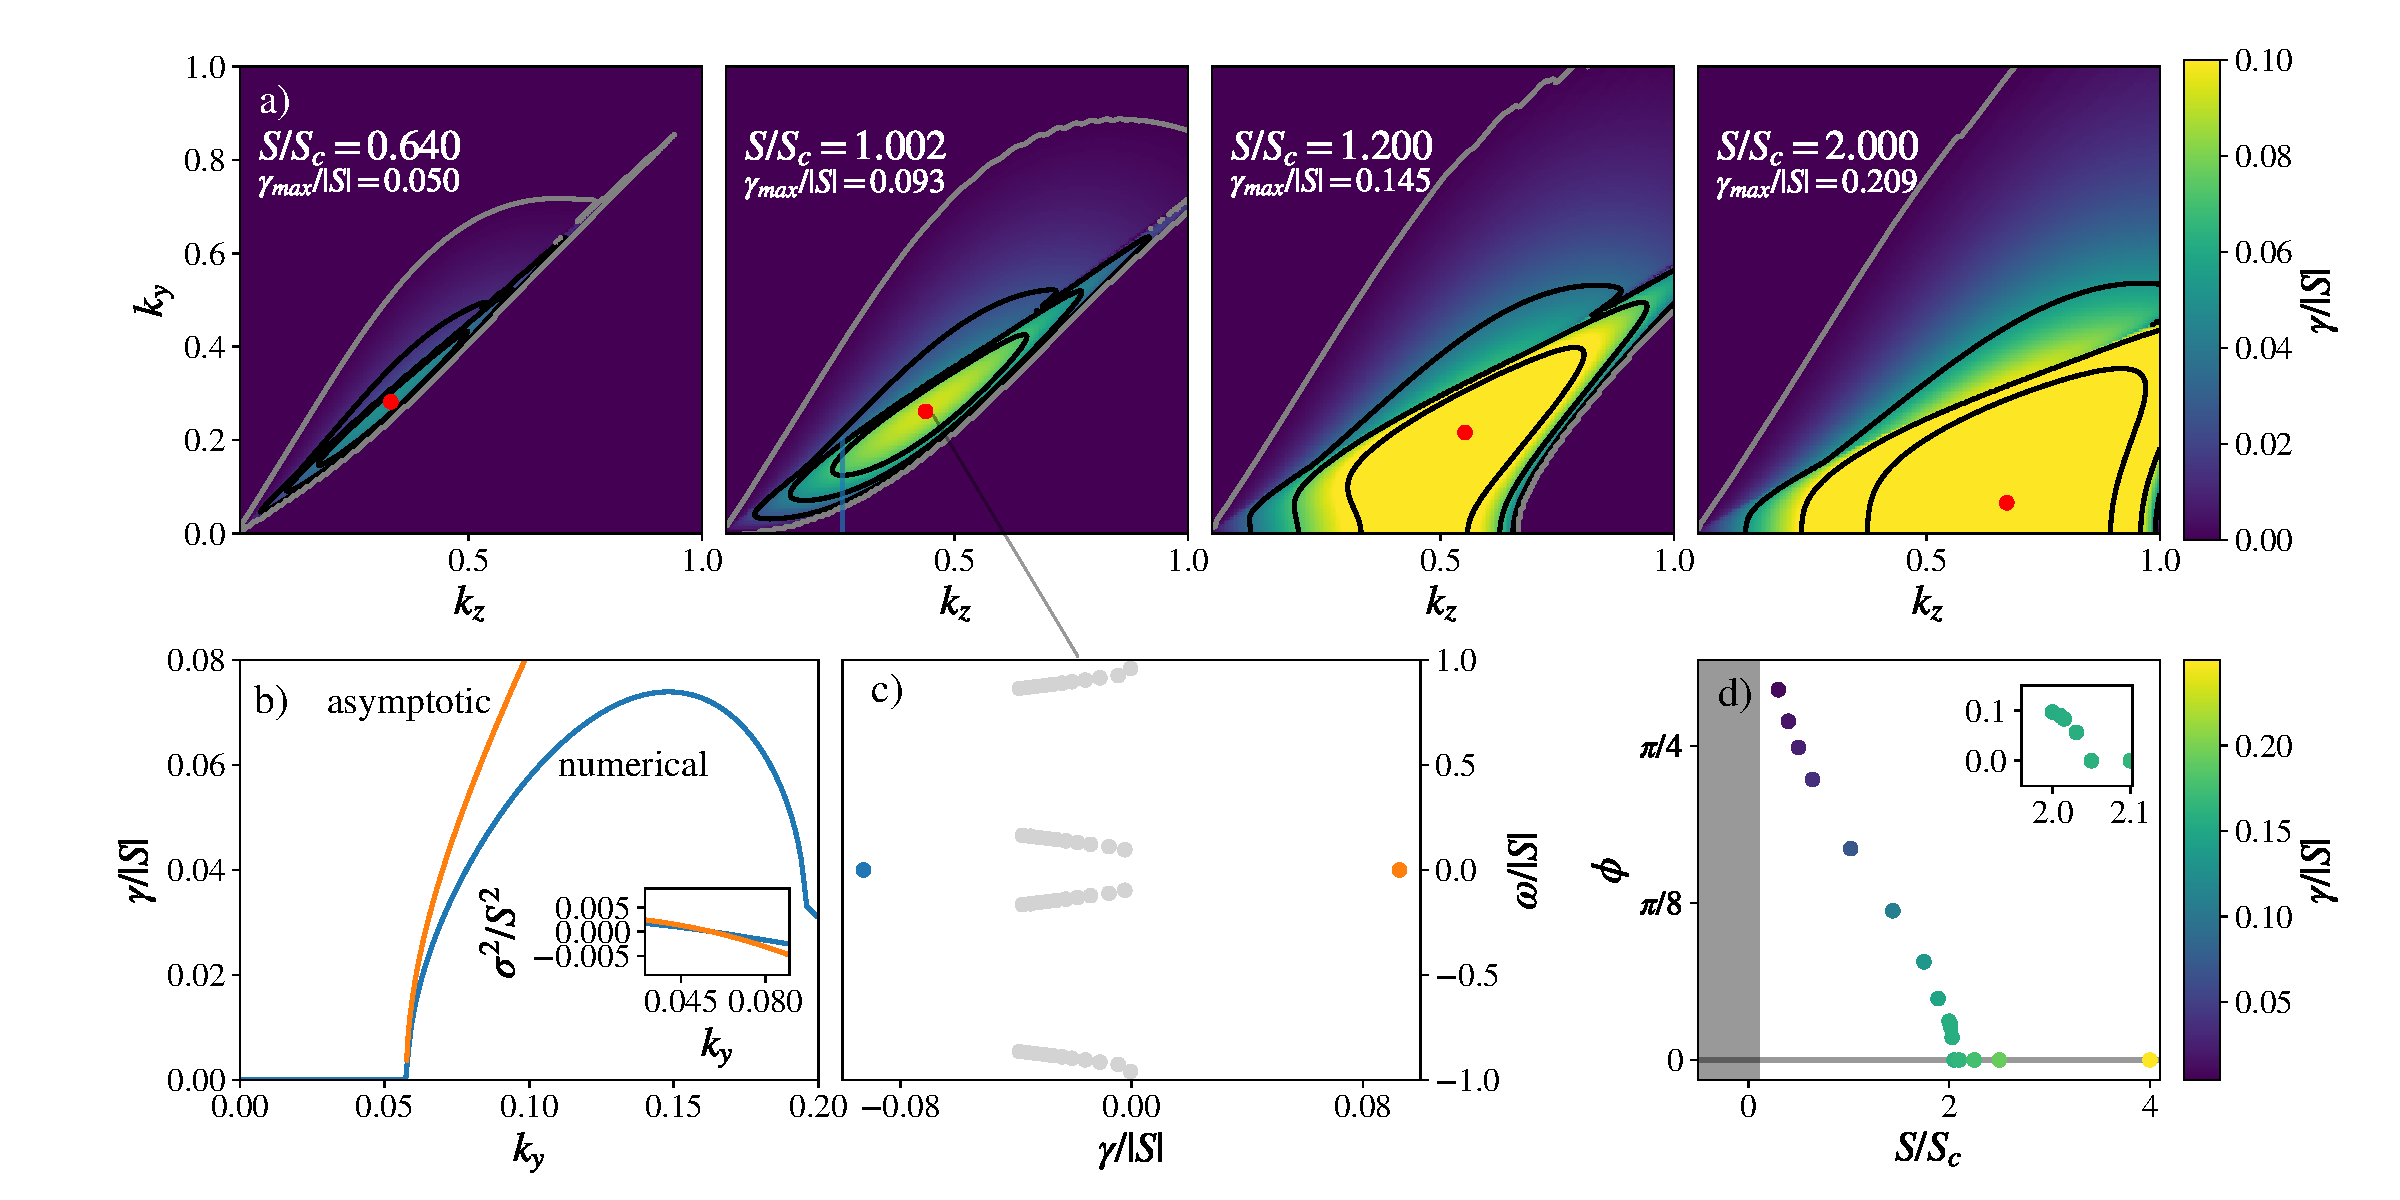
\includegraphics[width=\textwidth]{fig_1.pdf}
  \caption{Growth rates for three-dimensional MRI modes. a) growth rates $\gamma$ over a grid of $k_y$ and $k_z$ for four values of supercriticality $\SSC$. The white contour highlights $\gamma = 0$; the red dots indicate the fastest growing mode. At $\SSC = 0.640$, there are no two dimensional modes. b) Growth rate vs $k_y$ for $k_z = ???$ at $\SSC = 1.002$ (highlighted by the blue line in a). The orange line gives the asymptotic result from equation~(\ref{eq:asymp}) and the blue line are the numerical results. The asymptotic form is valid as $\SSC \to 1$ and $k_y \ll 1$. c) The full discrete spectrum of the MRI for $(k_y, k_z) \simeq (0.263, 0.447)$. The unstable mode is shown in orange; all other modes are stable ($\gamma \le 0$).}
  \label{fig:growth_rate}
\end{figure*}
%\twocolumngrid
%
Numerical simulations have consistently shown axisymmetric modes dominating early evolution of the MRI before breaking down into MHD turbulence \citep{1995ApJ...440..742H,2018ApJ...853..174H,2019ApJS..241...26D}. 
These axisymmetric modes, called ``channel modes,'' are exact non-linear solutions of the governing equations with shearing-periodic boundary conditions in $x$, and thus must saturate via parasitic modes from physics beyond non-linear mode coupling \citep{1994ApJ...432..213G}.
Though we use impenetrable, stress-free boundary conditions that do not allow the unbounded growth of channel modes, the basic principle that axisymmetric disturbences grow fastest is not clearly caused by boundary conditions.
thus, we must reconcile our results with those earlier simulations.
In figure~\ref{fig:alpha}, we plot the angle $\alpha = \arctan k_y/k_z$ of the fastest growing mode with the $z$ axis as function of $\SSC$.
Above $\SSC \gtrsim 2.05$, $\alpha$ is zero, indicating that axisymmetric modes have the fastest growth rates.
For the fiducial run in \citet{1996ApJ...464..690H}, $\SSC \simeq 4.84$ (similar values are found in most works).
Thus, our theory predicts that the linear dynamics should be dominated by axisymmetric modes for the parameters studied in prior numerical simulations.
%
\begin{figure}[h!]
  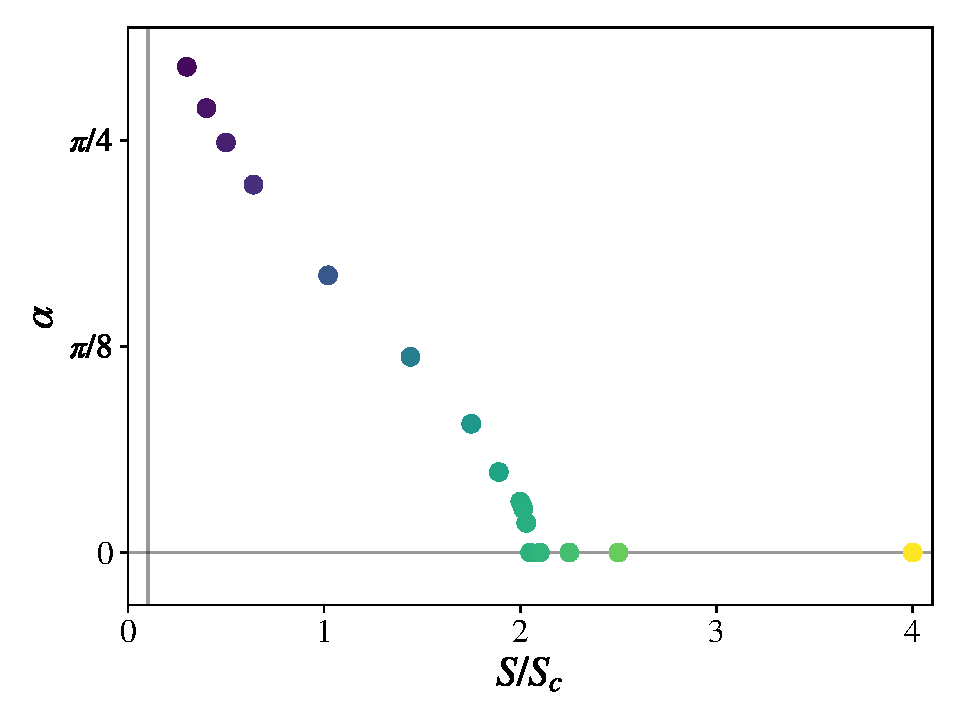
\includegraphics[width=\columnwidth]{alpha_vs_ssc_grid.pdf}
  \caption{Angle $\alpha$ of mode with respect to $z$ axis vs $\SSC$. The inset shows the transition from axisymmetric modes to three dimensional modes as $\SSC$ decreases below $2.05$. The shaded region indicates stability to all perturbations; the stability limit for three dimensional modes is $\SSC \simeq 0.102$.}
  \label{fig:alpha}
\end{figure}
%

However, even for $\SSC> 2.05$ there are significant swaths of unstable three-dimensional modes with growth rates comparable to the two-dimensional mode (figure~\ref{fig:growth_rate}a).
There are two significant implications for this.
First, the linear operator for the MRI, like other shearing systems, is non-normal; this effect appears whenever non-axisymmetric perturbations are allowed \citep[see][for a discussion relevant to the MRI]{1992MNRAS.255P..25K}.
Because of this, non-modal transient amplification occurs even for stable modes.
These effects can be strong enough to cause non-linear interactions and turbulence even when the entire flow is linearly stable.
While we are here concerned with systems linearly unstable to the MRI, the presence of three dimensional modes implies that linear, non-normal behavior could play a very strong role in the MRI near onset.

The second implication of the three dimensional modes is of considerably more importance.
These modes produce dynamo action in the linear regime, as evidenced by the presence of non-trivial eigenmodes for all three components of the magnetic field.
This is of considerable significance, as it leads to the possibility of a laminar MRI dynamo operating directly in regions of weak shear.
MRI dynamos have been studied in a number of different contexts \citep{2007PhRvL..98y4502R,2011ApJ...740...18O,2015PhRvL.114h5002S}, but all except one have focused on the turbulent dynamo. The lone exception, \citet{2016MNRAS.462..818B}, is a numerical study that discovered the exponential growth of mean magnetic fields during the linear growth phase of the MRI far from stability.
Our work explains this result in terms of purely linear dynamics:
non-axisymmetric MRI unstable modes drive the exponential growth of magnetic fields.

% \begin{itemize}
% \item non-normal and $k_y$ even when $\alpha = 0$ implies important role for linear dynamics at early times. 
% \item Following Squire + Bhattacharjee, this suggests that important stellar layers may in fact be driven by linear dynamics
% \item why is MRI non-oscillatory when hydro shear is oscil or stable?
% \end{itemize}

%If in two-column mode, this environment will change to single-column
% format so that long equations can be displayed. Use
% sparingly.
%\begin{widetext}
% put long equation here
%\end{widetext}

% figures should be put into the text as floats.
% Use the graphics or graphicx packages (distributed with LaTeX2e)
% and the \includegraphics macro defined in those packages.
% See the LaTeX Graphics Companion by Michel Goosens, Sebastian Rahtz,
% and Frank Mittelbach for instance.
%
% Here is an example of the general form of a figure:
% Fill in the caption in the braces of the \caption{} command. Put the label
% that you will use with \ref{} command in the braces of the \label{} command.
% Use the figure* environment if the figure should span across the
% entire page. There is no need to do explicit centering.

% \begin{figure}
% \includegraphics{}%
% \caption{\label{}}
% \end{figure}

% Surround figure environment with turnpage environment for landscape
% figure
% \begin{turnpage}
% \begin{figure}
% \includegraphics{}%
% \caption{\label{}}
% \end{figure}
% \end{turnpage}

% tables should appear as floats within the text
%
% Here is an example of the general form of a table:
% Fill in the caption in the braces of the \caption{} command. Put the label
% that you will use with \ref{} command in the braces of the \label{} command.
% Insert the column specifiers (l, r, c, d, etc.) in the empty braces of the
% \begin{tabular}{} command.
% The ruledtabular enviroment adds doubled rules to table and sets a
% reasonable default table settings.
% Use the table* environment to get a full-width table in two-column
% Add \usepackage{longtable} and the longtable (or longtable*}
% environment for nicely formatted long tables. Or use the the [H]
% placement option to break a long table (with less control than 
% in longtable).
% \begin{table}%[H] add [H] placement to break table across pages
% \caption{\label{}}
% \begin{ruledtabular}
% \begin{tabular}{}
% Lines of table here ending with \\
% \end{tabular}
% \end{ruledtabular}
% \end{table}

% Surround table environment with turnpage environment for landscape
% table
% \begin{turnpage}
% \begin{table}
% \caption{\label{}}
% \begin{ruledtabular}
% \begin{tabular}{}
% \end{tabular}
% \end{ruledtabular}
% \end{table}
% \end{turnpage}

% Specify following sections are appendices. Use \appendix* if there
% only one appendix.
%\appendix
%\section{}

% If you have acknowledgments, this puts in the proper section head.
\begin{acknowledgments}
We would like to thank Steve Tobias for helpful conversations on this work.
JSO acknowledges funding from NASA LWS grant No. NNX16AC92G and Research Corporation Scialog Collaborative Award (TDA) ID\#24231. Computations were performed on the \emph{Leavitt} cluster at the Bates College High Performance Computing Center.
Morgan Baxter acknowledges support from NASA LWS grant No. NNX16AC92G.
\end{acknowledgments}

% Create the reference section using BibTeX:
\bibliography{mri}

\end{document}
%
% ****** End of file apstemplate.tex ******

